\documentclass[../RelazioneFinale.tex]{subfiles}

\lstdefinestyle{sharpc}{language=[Sharp]C,frame=single, rulecolor=\color{white}, backgroundcolor=\color{white!98!black}}
						\lstset{style=sharpc}


\begin{document}

	\chapter{Dettagli componenti}
	\label{cap:Dettagli}
		
		Nel seguente capitolo si presentano i dettagli implementativi ritenuti più interessanti e utili delle macro componenti presentate in precedenza.
		La lettura di questa parte può essere utilizzata come approfondimento della parte architetturale o come approfondimenti indipendenti sullo sviluppo di parti del sistema Updater.
		Di seguito vengono presentate le sezioni accompagnate da una breve descrizione.
		\begin{itemize}
			\item Updater - Parte client;
			\begin{itemize}
				\item \textbf{Interfaccia grafica \ref{subsec:InterfacciaGrafica}}: descrive attraverso le immagini le componenti grafiche che compongono l'interfaccia grafica del programma Updater;
				\item \textbf{Flusso principali operazioni \ref{subsec:operazioni}}: descrive attraverso l'uso di diagrammi di attività gli algoritmi che effettuano le operazioni principali;
			\end{itemize}
			\item Updater - parte server;
			\begin{itemize}
				\item \textbf{Sito web amministrativo \ref{sec:SitoWeb}}: descrive come è costruito il sito web e come sono usate le tecnologie;
				\item \textbf{Web Api documentazione \ref{subsec:WebApi}}: documenta l'uso degli uri per effettuare richieste al servizio REST;
			\end{itemize}
			\item \textbf{Concorrenza \ref{sec:Concorrenza}}: descrive come è gestita la concorrenza all'interno del programma Updater e il pattern utilizzato;
			\item \textbf{PowerShell script \ref{sec:PSscript}}: descrive lo script che permette il collegamento tra il sistema di \emph{continuos integration} e il sistema Updater sviluppato.
		\end{itemize}
	
		%\section{Updater Client Library - Documentazione}
		\label{sec:UpdaterClientLibrary}
		
			\subsection{Introduzione}
			
			
			\subsection{Componenti}
			
				\subsubsection{Indice componenti}
				
				\begin{tabular}{lc}
					nome classe & pagina \\
					MyClass & \pageref{MyClass} \\
					\verb|UpdaterService| & \pageref{} \\
					\verb|ProductWrapper| & \pageref{} \\
					\verb|PrerequisiteWrapper| & \pageref{} \\
					\verb|AutomaticUpdatesController| & \pageref{} \\
					\verb|AutomaticUpdatesInstaller| & \pageref{} \\
					\verb|AutomaticUpdatesCheckerAndDownloader| & \pageref{} \\
					\verb|AppRestarter| & \pageref{} \\
					\verb|Models::ObjectManager| & \pageref{} \\
				
				\end{tabular}
				
				\subsubsection{ProductWrapper}

					\begin{figure}
						%\includegraphics[scale=•]{•}
					\end{figure}									
				
					\paragraph{Responsabilità}
					
					\paragraph{Descrizione metodi} \ \par
					
						%\hspace{4cm}
						
						\begin{lstlisting}
 main(stringa : string, secondo : Tipo) : void
						\end{lstlisting}
						Bla blas bla 
						
						\begin{lstlisting}
 void main2(VarArgs...args)
						\end{lstlisting}
				
					
				\subsubsection{PrerequisiteWrapper}
				
					%\begin{figure}
						%\includegraphics[scale=•]{•}
					%\end{figure}								
				
					\paragraph{Responsabilità}
					
					\paragraph{Descrizione metodi} \ \par
					
						
						\begin{lstlisting}
 main(stringa : string, secondo : Tipo) : void
						\end{lstlisting}
						Bla blas bla 
						
						\begin{lstlisting}
 void main2(VarArgs...args)
						\end{lstlisting}
	
		\paragraph*{}
		\label{MyClass}
		\begin{tcolorbox}[fonttitle=\bfseries, 
								adjusted title={\Large MyClass}, 
								breakable, 
								sharp corners=south,
								colback=white, 
								colframe=white!60!black]
								
				\begin{description}%[leftmargin=0.7cm,labelwidth=!]
				
					\item[Responsabilità] \ \par 
        				asnfogandgonadonfkln fjsdnf kans njsdf nkajsnf 
        				
        			\tcbline 
        				
        			\item[Descrizione metodi] \ \par
        				
        				\begin{lstlisting}
 main(stringa : string, secondo : Tipo) : void
						\end{lstlisting}
						Bla blas bla 
						
						\begin{lstlisting}
 void main2(VarArgs...args)
						\end{lstlisting}
        				
				\end{description}  
				
			\end{tcolorbox}	
	
		\paragraph*{}
		\label{AppRestarter}
		\begin{tcolorbox}[fonttitle=\bfseries, 
								adjusted title={\Large AppRestarter}, 
								breakable, 
								sharp corners=south,
								colback=white, 
								colframe=white!60!black]
								
				\begin{description}%[leftmargin=0.7cm,labelwidth=!]
				
					\item[Responsabilità] \ \par 
        				Gestire la funzionalità di riavvio dell'applicazione come amministratore per le operazioni:
        				\begin{itemize}
        					\item Aggiornamenti;
        					\item Installazioni;
        					\item Operazioni automatiche in background.
        				\end{itemize}
        			\tcbline 
        				
        			\item[Descrizione metodi] \ \par
        				
        				\begin{lstlisting}
public AppRestarter()
						\end{lstlisting}
						Costruttore della classe.
						
						\begin{lstlisting}
bool IsAppRunningAsAdministrator()
						\end{lstlisting}
						Metodo per conoscere se l'applicazione è già in esecuzione con i permessi d'amministratore.
						
						\begin{lstlisting}
void RestartAppAsAdminForUpdate(long idProduct)
						\end{lstlisting}
						Metodo per riavviare l'applicazione con i permessi d'amministratore gestendo gli aggiornamenti del prodotto software indicato nel parametro \verb|idProduct|.  
						
						\begin{lstlisting}
void RestartAppAsAdminForInstall(long idProduct)
						\end{lstlisting}
						Metodo per riavviare l'applicazione con i permessi d'amministratore gestendo l'installazione del prodotto software indicato nel parametro \verb|idProduct|.  	
						
						\begin{lstlisting}
void RestartAppAsAdminForBackgroundOperation
			    (long idProduct)
						\end{lstlisting}
						Metodo per riavviare l'applicazione con i permessi d'amministratore gestendo operazioni in background (download, installazione e aggioramento) del prodotto software indicato nel parametro \verb|idProduct|.  					
        				
				\end{description}  
				
			\end{tcolorbox}	


\newpage % -----------------------------------------------------
		
	\section{Updater - Parte client}
		
		\subsection{Interfaccia grafica}
		\label{subsec:InterfacciaGrafica}
			L'interfaccia grafica sviluppata per il programma Updater attualmente è in uno stato \textbf{prototipale}, ogni immagine presentata è usata come riferimento per indicare come l'utente può usufruire delle funzionalità del programma.
			
			\subsubsection{Componenti}
			Il programma Updater è costituito dalla finestra principale creata dall'oggetto:
			\begin{quote}
				 \verb|MainWindow|;
			\end{quote}
			La quale è costituita da tre elementi grafici i quali ne racchiudono altri resi disponibili dal framework WPF e per questo non considerati. Essi sono:
			\begin{enumerate}
				\item \verb|ProductsListView|;
				\item \verb|ProductControlView|;
				\item \verb|ProductInfoView|.
			\end{enumerate}
			Nella figura \ref{fig:MainWindowComponents} sono evidenziati e indicati attraverso la corrispondenza del numero dell'elenco precedente.
			
			\begin{figure}[h]
				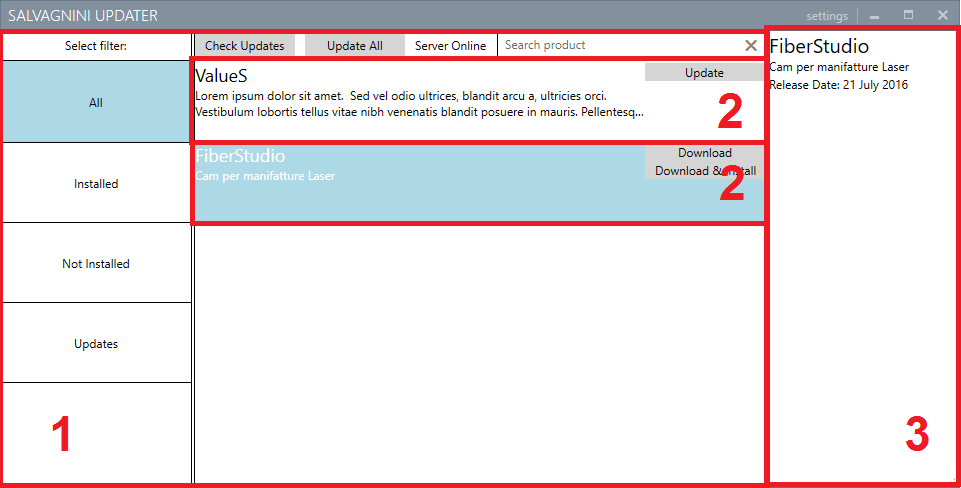
\includegraphics[width=\textwidth]{UpdaterUI/MainWindowComponents}
				\caption{Componenti grafiche della finestra principale}
				\label{fig:MainWindowComponents}
			\end{figure}
			
			È inoltre presente una schermata delle impostazioni del programma che si sovrappone agli elementi grafici \ref{fig:Client-Settings}, essa è definita nel componente \verb|SettingsView|.
			
\newpage
			\subsubsection{Funzionalità}
			La schermata principale (figura \ref{fig:Client-Main}) permette subito di avere la lista dei prodotti software interagendo su di essi attraverso alla lista di pulsanti relativa. Questa cambia rendendo disponibili diversi pulsanti in base allo stato del prodotto software.
			Alla sinistra è possibile filtrare la lista di prodotti software mentre in alto al centro è possibile filtrarla attraverso la ricerca del nome all'interno della casella di ricerca. Sempre in alto è possibile trovare i pulsanti:
			\begin{description}
				\item[Check Updates] che aggiorna la lista dei prodotti software attraverso una nuova richiesta al server;
				\item[Update All] che aggiorna tutti i prodotti software che hanno aggironamenti disponibili pendenti.
			\end{description}
			Alla sinistra invece troviamo uno spazio disponibile a mostrare tutti i dati disponibili di un prodotto software.
			
			
			Tramite il click della parola \emph{Settings} situata in alto a sinistra è possibile aprire una schermata che si sovrappone agli elementi grafici (figura \ref{fig:Client-Settings}). Da qui è possibile impostare l'esecuzione automatica di alcune funzionalità.

			\hspace{2cm}			
			
			\begin{figure}[h]
				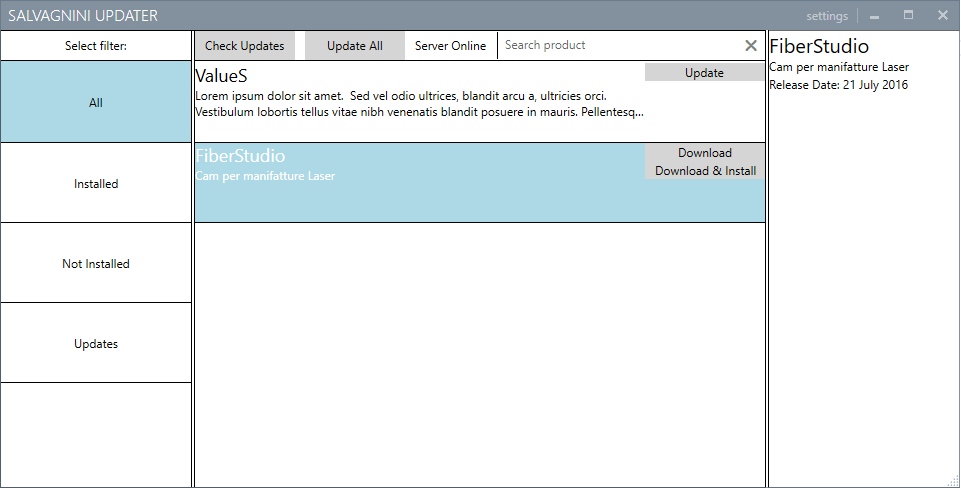
\includegraphics[width=\textwidth]{UpdaterUI/Client-Main}
				\caption{Updater - Finestra principale}
				\label{fig:Client-Main}
			\end{figure}
		
\newpage	
			
			\begin{figure}[h]
				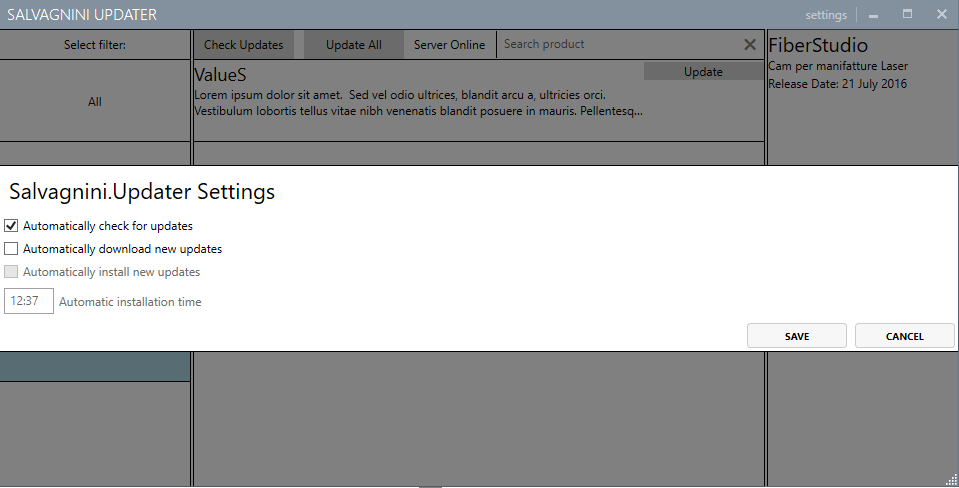
\includegraphics[width=\textwidth]{UpdaterUI/Client-Settings}
				\caption{Updater - Schermata delle impostazioni}
				\label{fig:Client-Settings}
			\end{figure}	

		\subsection{Flusso d'esecuzione operazioni principali}
		\label{subsec:operazioni}
			Di seguito vengono presentati i diagrammi di attività che mostrano in dettaglio i passaggi che la logica del programma effettua alla richiesta di esecuzione delle seguenti operazioni:
			\begin{itemize}
				\item Download (figura \ref{fig:Download});
				\item Installazione (figura \ref{fig:Installazione});
				\item Aggiornamento (figura \ref{fig:Aggiornamento});
				\item Reinstallazione;
				\item Download e installazione;
			\end{itemize}
			
			In particolare si vuole mostrare nel modo più chiaro possibile come si sia risolto il problema della gestione dei prerequisiti prima dell'installazione di un prodotto software che li richiede.
			I diagrammi manterranno nella colonna centrale il flusso con i casi peggiori. Per i diagrammi \emph{``Reinstallazione''} e \emph{``Download e installazione''} si veda il diagramma \emph{``Aggiornamento''} (figura \ref{fig:Aggiornamento}).
			
			\begin{figure}[p]
				\centering
				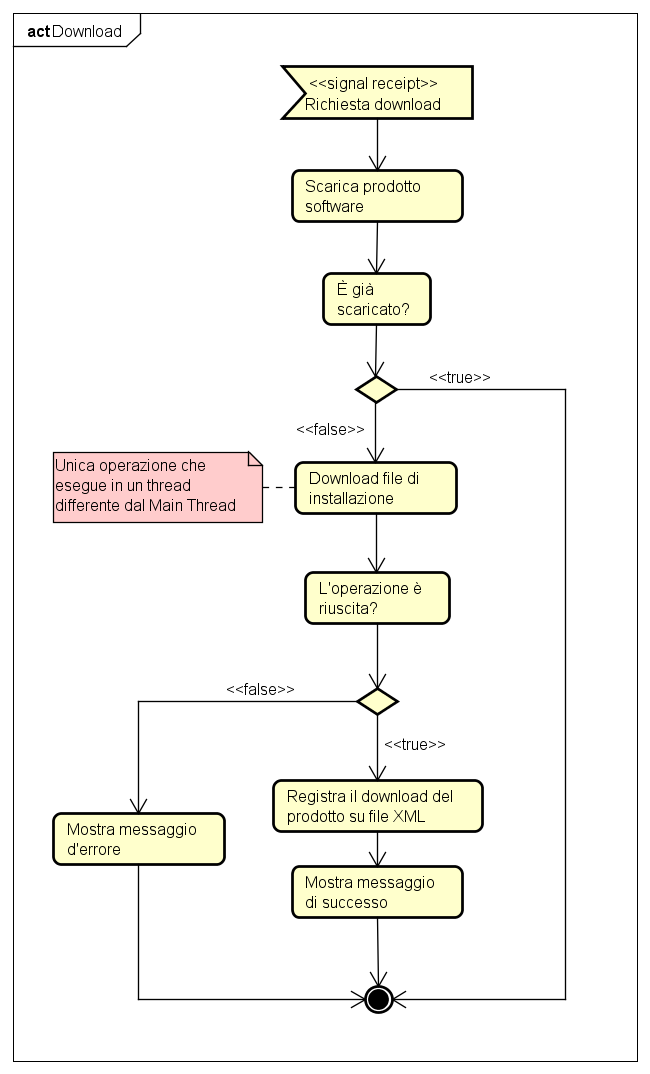
\includegraphics[width=\textwidth]{Download}
				\caption{Diagramma di attività - Download}
				\label{fig:Download}
			\end{figure}
			
			\begin{figure}[p]
				\centering
				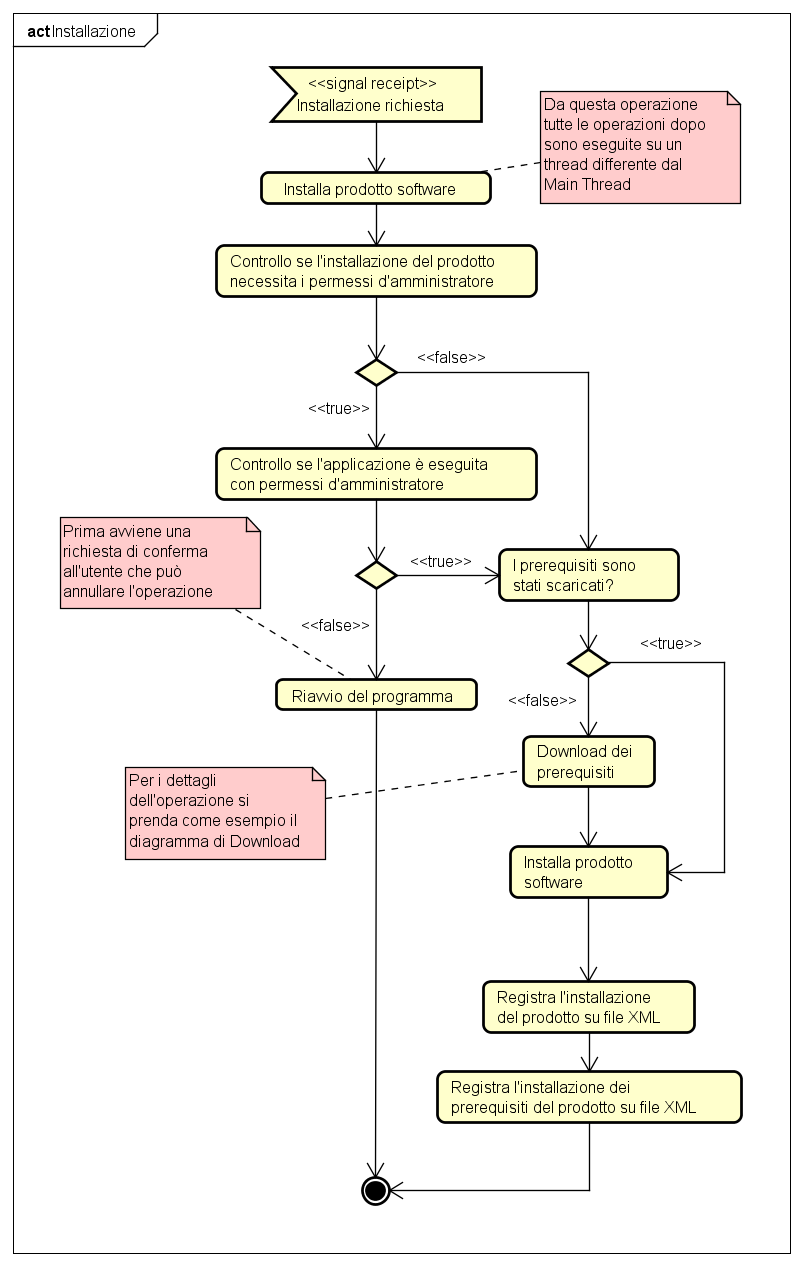
\includegraphics[width=\textwidth]{Installazione}
				\caption{Diagramma di attività - Installazione}
				\label{fig:Installazione}
			\end{figure}
			
			\begin{figure}
				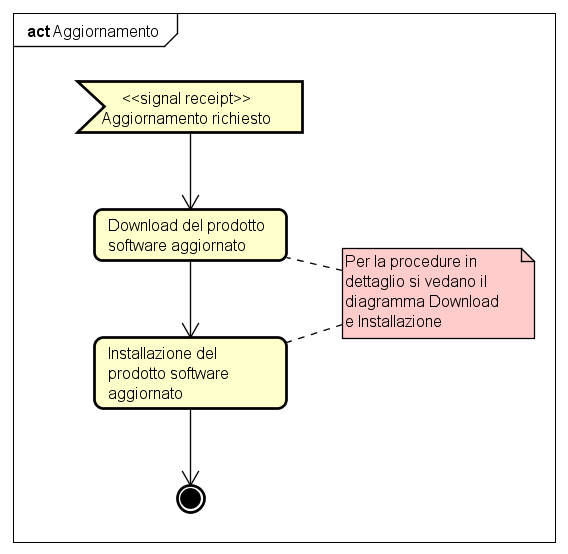
\includegraphics[width=\textwidth]{Aggiornamento}
				\caption{Diagramma di attività - Aggiornamento}
				\label{fig:Aggiornamento}
			\end{figure}
		
		
\newpage % -----------------------------------------------------

		\section{Updater - Parte server}
		
			\subsection{Sito web amministrativo}
			\label{sec:SitoWeb}
				Per semplificare e agevolare le modifiche alla base di dati si è costruito un piccolo sito web costituito da quattro pagine web composte con elementi di Bootstrap e rese dinamiche grazie all'uso di Javascript con la libreria KnockoutJs.
				
				\subsubsection{Pagine web}
				\begin{description}
					\item[Login.html] permette l'autenticazione per accedere alle altre pagine;
					\item[Products.html] permette di aggiungere, eliminare o modificare un prodotto software (figura \ref{fig:Products}).
					\item[Prerequisites.html] permette di aggiungere, eliminare o modificare un prerequisito software (figura \ref{fig:Prerequisites}).
					\item[Dependencies.html] permette di associare e dissociare i prodotti software dai prerequisiti software (figura \ref{fig:Dependencies}).
				\end{description}
				
				\begin{figure}[p]
					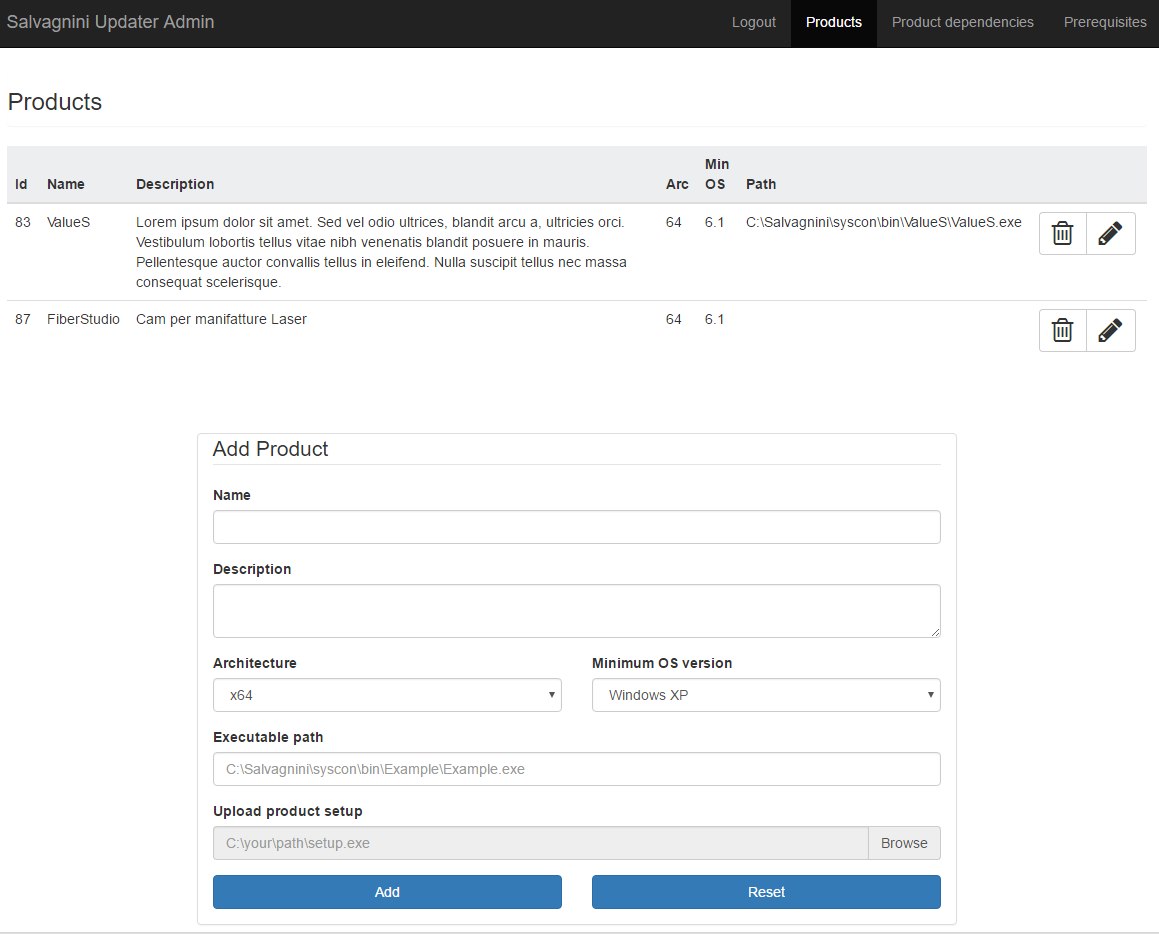
\includegraphics[width=\textwidth]{WebUI/Products}
					\caption{Pagina web - Products.html}
					\label{fig:Products}
				\end{figure}
		
				\begin{figure}[p]
					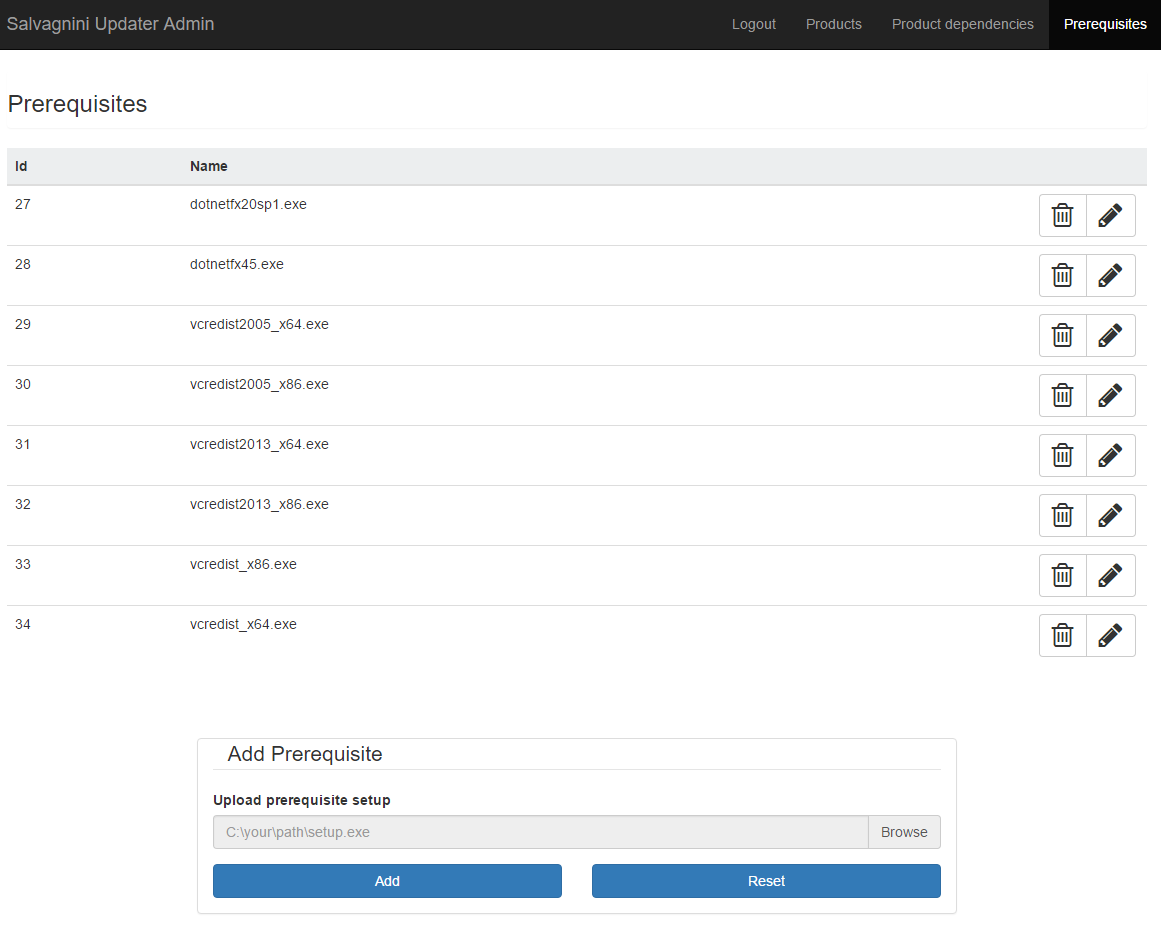
\includegraphics[width=\textwidth]{WebUI/Prerequisites}
					\caption{Pagina web - Prerequisites.html}
					\label{fig:Prerequisites}
				\end{figure}
				
				\begin{figure}[p]
					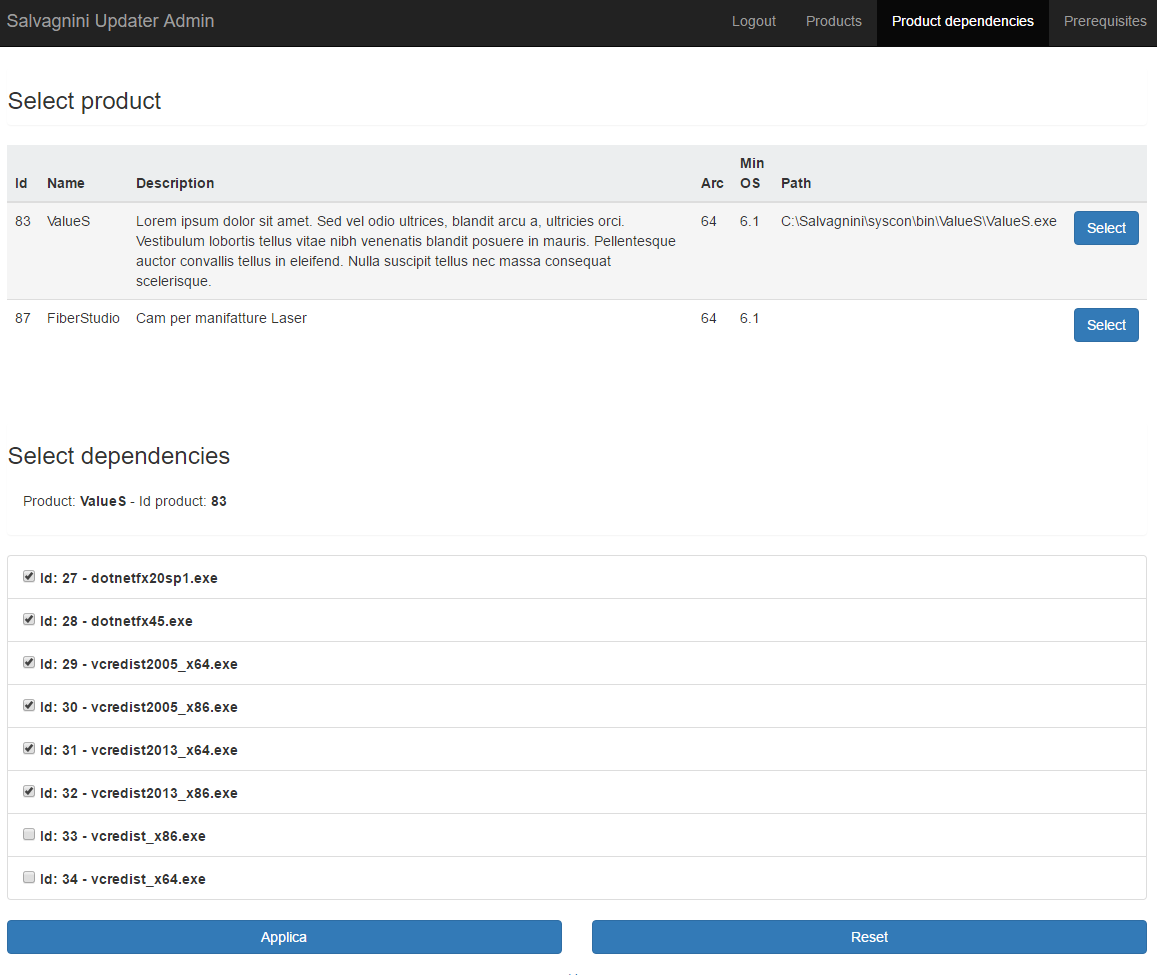
\includegraphics[width=\textwidth]{WebUI/Dependencies}
					\caption{Pagina web - Dependencies.html}
					\label{fig:Dependencies}
				\end{figure}							
\newpage				
				\subsubsection{Script Javascript}
					Per rendere le pagine web dinamiche si è utilizzato l'attributo \verb|data-binding| di HTML5 e la libreria KnockoutJs che lo gestisce.
					Per ogni pagina si è codificato il relativo file di script più un file \verb|Common.js| che contiene funzioni utilizzate in tutte le pagine.
					
					La struttura degli script è la seguente:
					\begin{enumerate}
					
						\item Si assegna all'elemento HTML l'attributo \verb|data-bind| al cui interno vengono usate keyword che Knockout riconosce e interpreta. Ad esempio:
						\begin{lstlisting}[language=html]
<p data-bind="text:message"></p>
						\end{lstlisting}
						
						\item A questo punto sul file script associato alla pagina si crea un oggetto che rappresenta il ViewModel di quella pagina web:
						\begin{lstlisting}[language=Javascript]
var ViewModel = function () {
	// ...
}

ko.applyBindings(new ViewModel);
						\end{lstlisting}
						
						\item All'interno del ViewModel saranno codificati i campi dati e i metodi che agiranno agli input dell'utente nella pagina html. Per rendere l'aggiornamento dei dati (\emph{data-binding}) automatico è sufficiente definire i campi dati del ViewModel con un costrutto offerto dalla libreria (il nome delle variabili deve corrispondere alla stringa inserita nel data-bind delle pagine web):
						\begin{lstlisting}[language=Javascript]
var message = ko.observable();
						\end{lstlisting}
						
						\item Ora qualsiasi cambiamento sul valore della variabile \verb|message| sarà automaticamente riflesso nella pagina web.
					\end{enumerate}
				
	
\newpage 
		
			\subsection{Web Api - Documentazione}
			\label{subsec:WebApi}
				Di seguito si elencano i \textbf{controller} definiti nella costruzione del servizio REST Updater Server. Per ogni controller vengono elencati gli indirizzi uri per poter effettuare una richiesta HTTP.
				Le tipologie di richieste HTTP supportate sono:
				\begin{itemize}
					\item Get: alla richiesta viene risposto restituendo dati;
					\item Post: alla richiesta vengono processati i dati contenuti in essa, se conformi vengono salvati nella base di dati;
					\item Delete: alla richiesta viene effettuata una cancellazione definitiva dei dati indicati;
					\item Put: alla richiesta vengono processati i dati contenuti in essa, se conformi vengono salvati nella base di dati sovrascrivendo quelli indicati.
				\end{itemize}
				
				La trasmissione dei dati avviene attraverso la serializzazione in formato JSON.
		
			\subsubsection{ProductsController}
			\begin{description}
			
				\item Operazioni GET:
				\begin{itemize}
				
					\item \verb|api/Products| 
					\item[] Restituisce tutti i prodotti software all'interno della base di dati;
					
					\item \verb|api/Products/{id}| 
					\item[] Restituisce il prodotto software identificato dall'\verb|id| indicato;
					
					\item \verb|api/Products/{productId}/Prerequisites|
					\item[] Restituisce la lista di prerequisiti software del prodotto identificato da \verb|productId|;
					
					\item \verb|api/Products/check/{id}/{fileName}|
					\item[] Restituisce vero se il prodotto software identificato dall'\verb|id| indicato ha il \verb|fileName| indicato altrimenti falso;
					
				\end{itemize}			
				
				\item Operazioni PUT:
				\begin{itemize}
				
					\item \verb|api/Products/{id}|
					\item[] Sovrascrive con nuovi dati le informazioni associate al prodotto software identificato dall'\verb|id| indicato;
					
				\end{itemize}								
				
				\item Operazioni POST:
				\begin{itemize}
					\item \verb|api/Products|
					\item[] Aggiunge un prodotto software con i dati contenuti nella richiesta;
					
					\item \verb|api/Products/{productId}/Prerequisites|
					\item[] Associa i prerequisiti contenuti nella richiesta al prodotto software identificato dal \verb|productId| indicato. Dopo l'operazione solo i prerequisiti segnalati saranno associati al prodotto;
					
				\end{itemize}

				\item Operazioni DELETE:
				\begin{itemize}
					\item \verb|api/Products/{id}| 
					\item[] Elimina il prodotto software identificato dall'\verb|id| indicato.
				\end{itemize}
				
			\end{description}						
			
			\subsubsection{PrerequisiteController}
			\begin{description}
				\item Operazioni GET:
				\begin{itemize}
					\item \verb|api/Prerequisites|
					\item[] Restituisce tutti i prerequisiti software all'interno della base di dati;
					\item \verb|api/Prerequisites/check/{id}/{fileName}|
					\item[] Restituisce vero se il prodotto software identificato dall'\verb|id| indicato ha il \verb|fileName| indicato altrimenti falso;
					\item \verb|api/Prerequisites/check/{id}/hasDependencies|
					\item[] Restituisce vero se il prerequisito software identificato dall'\verb|id| indicato è associato almeno ad un prodotto software;
									
				\end{itemize}
				
				\item Operazioni PUT:
				\begin{itemize}
					\item \verb|api/Prerequisites/{id}| 
					\item[] Sovrascrive con nuovi dati le informazioni associate al prerequisito software identificato dall'\verb|id| indicato;
				\end{itemize}								
	
				\item Operazioni POST:
				\begin{itemize}
					\item \verb|api/Prerequisites|
					\item[] Aggiunge un prerequisito software con i dati contenuti nella richiesta;
				\end{itemize}				
				
				\item Operazioni DELETE:
				\begin{itemize}
					\item \verb|api/Prerequisites/{id}|
					\item[] Elimina il prerequisito software identificato dall'\verb|id| indicato.
				\end{itemize}
				
			\end{description}

		
			
\newpage % -----------------------------------------------------
	
		\section{Concorrenza}
		\label{sec:Concorrenza}
			La concorrenza ha coinvolto solamente la parte client del sistema sviluppato. La necessità di ricorrere alla concorrenza giunge quando si vuole rendere la propria applicazione responsive, ossia non impegnare il Main Thread, definito anche come UI Thread, in operazioni lunghe mostrando di fatto all'utente l'interfaccia grafica bloccata.
			Mostrare all'utente l'interfaccia bloccata non è mai buona pratica, l'utente infatti traduce questo feedback in qualcosa del tipo: \emph{"l'applicazione si è bloccata"} e non \emph{"L'applicazione sta elaborando qualcosa per te"}.
			Per questo motivo nella parte client del sistema si è deciso di inserire multipli thread, e incapsulare le elaborazioni più complesse in task.
			\subsection{Pattern}
				In \Csharp\ esistono vari pattern per l'esecuzione di un ambiente concorrente, l'ultimo di questi, nonché quello consigliato dalla stessa Microsoft\footnote{\emph{Stephen Toub, Asynchronous Programming Patterns} \url{https://msdn.microsoft.com/it-it/library/jj152938(v=vs.110).aspx}} e scelto per il progetto, è il \emph{Task-based Asynchronous Pattern} (TAP).
				
				\subsubsection{Applicazione Task-based Asynchronous Pattern}
				Esso si basa sui tipi \verb|Task| e \verb|Task<TResult>| definiti all'interno del namespace \verb|System.Threading.Tasks| che sono utilizzati per rappresentare operazioni asincrone.
				Il pattern permette una notevole semplificazione nella codifica per introdurre codice concorrente, inoltre attraverso l'uso delle keyword \verb|async| e \verb|await|, parte del linguaggio \Csharp\ è molto più facile capire quali porzioni di codice sono eseguite concorrentemente e quali no.
				La definizione di un metodo asincrono sarà di questo tipo:
				\begin{lstlisting}
public async Task<TResult> AsyncMethod(Type param)
				\end{lstlisting}
				e potrà essere chiamato attraverso l'uso di \verb|await|:
				\begin{lstlisting}
var returnValue = await AsyncMethod(param);
				\end{lstlisting}
				la concorrenza viene creata attraverso l'uso del metodo statico \verb|Task.Run()|:
				\begin{lstlisting}
var returnValue = await Task.Run(() => AsyncMethod()));				
				\end{lstlisting}
				Da qui in poi tutti i metodi definiti \verb|async| a partire da AsyncMethod() saranno eseguiti in un thread differente dal Main Thread.
				
			\subsection{Componenti coinvolte}
				Di seguito si elencano le componenti e i relativi metodi che includono la concorrenza:
				\begin{itemize}
					\item[] \verb|ProductWrapper|: \lstinline|InitializePrerequisitesWrapper()|;
					\item[] \verb|ProductWrapper|: \lstinline|Download()| (attraverso l'uso della classe \verb|WebClient| di .NET);
					\item[] \verb|ProductsPanelModel|: \lstinline|LoadProduct()|;
					\item[] \verb|ProductControlModel|: \lstinline|InstallProduct()|.
				\end{itemize}
			
			In generale, nell'implementazione si sono seguite queste linee guida:
				\begin{itemize}
					\item Qualsiasi operazione che richiede l'accesso alla rete è asincrona;
					\item Le operazioni che non richiedono l'accesso a internet ma comunque necessitano di tempo per i calcoli sono asincrone e sono contenute esclusivamente nel macro componente \emph{Updater UI Controls};
				\end{itemize}
				
			\subsection{Criticità e miglioramenti}
				Fortunatamente le operazioni da eseguire in concorrenza non riportano i problemi di accessi condivisi a risorse e questo ha semplificato l'implementazione. Ciononostante la \emph{best practice} di mantenere separato il codice concorrente dal codice non concorrente non è seguita. Seppur le componenti che includono l'avvio di nuovi task sono poche e i casi in cui si verifica sono limitati a quelli elencati precedentemente la linea di codice:
				\begin{lstlisting}
returnValue = await Task.Run(() => object.Method()));				
				\end{lstlisting}
		non risulta mai ben isolata dal resto del codice sincrono.
		
		Una più corretta soluzione sarebbe quella di incorporare l'avvio di nuovi task all'interno di singoli oggetti ben definiti in cui è chiaramente visibile l'implementazione della concorrenza.
			
			\subsection{Approfondimenti}
			\begin{itemize}
				\item Stephen Cleary, \emph{Async \&\ Await} \url{http://blog.stephencleary.com/2012/02/async-and-await.html};
				\item Stephen Cleary, \emph{Asyncronous Programming Best Practices} \url{https://msdn.microsoft.com/magazine/jj991977.aspx};
				\item Stephen Toub, \emph{Task-based Asynchronous Pattern}, disponibile al seguente indirizzo \url{https://www.microsoft.com/en-us/download/details.aspx?id=19957};
				
				\item Stephen Cleary, \emph{Concurrency in \Csharp\ Cookbook}.
			\end{itemize}


\newpage % ---------------------------------------------------

	\section{PowerShell script}
	\label{sec:PSscript}
		Nella presente sezione viene presentato e descritto lo script powershell che si occupa di automatizzare l'aggiornamento dei prodotti software all'interno della base di dati.
		
		\subsection{Ambito applicativo dello script}
			Il sistema di \emph{Continuos Integration} (CI) aziendale consente di definire dei processi per la compilazione del codice, l'esecuzione dei test e l'esecuzione di script batch.
			L'aggiornamento di un prodotto software attraversa i seguenti passaggi:
			\begin{enumerate}
				\item \textbf{Commit} dello sviluppatore nel repository;
				\item \textbf{Esecuzione processo} definito nella piattaforma di \textbf{CI} (solitamente compilazione ed esecuzione dei test);
				\item \textbf{Creazione dell'eseguibile binario} di installazione del prodotto se il passaggio precedente non ha riscontrato errori;
			\end{enumerate}
			A questo punto entra in gioco la nuova parte sviluppata:
			\begin{enumerate}
				\setcounter{enumi}{3}
				\item \textbf{Esecuzione} di uno \textbf{script batch}, il quale contiene gli input per lo script powershell;
				\item \textbf{Esecuzione} dello \textbf{script powershell}. A questo punto lo script esegue una normale richiesta PUT al servizio REST e aggiorna il prodotto specificato dagli input in ingresso.
			\end{enumerate}
		
		\subsection{Implementazione script powershell}
			\subsubsection*{Input richiesti}
			\begin{itemize}
				\item \verb|$InFile|: il percorso dell'eseguibile per l'installazione;
				\item \verb|$uri|: l'indirizzo per effettuare la richiesta PUT al server;
				\item \verb|$user|: il nome utente per l'autenticazione della richiesta;
				\item \verb|$pass|: la password per l'autenticazione della richiesta.
			\end{itemize}
			
			\subsubsection*{Dipendenze esterne con .NET}
			\begin{itemize}
				\item \verb|System.Web|
				\item \verb|System.Net.Http|
			\end{itemize}
			
			\subsubsection*{Logica operativa}
				La logica operativa segue la costruzione di una richiesta HTTP di tipo PUT con autorizzazione base:
				\begin{enumerate}
					\item Defizione dell'autorizzazione base attraverso la coppia username e password per l'invio della richiesta HTTP;
					\item Costruzione \verb|ContentDispositionHeaderValue| di tipo \emph{form-data} e inserimento del file e del suo nome;
					\item Costruzione dell'header della richiesta HTTP inserendo all'interno l'oggetto precedentemente creato: \verb|ContentDispositionHeaderValue|;
					\item Invio della richiesta HTTP.
				\end{enumerate}
			
		%\subsection{Approfondimenti}
			
	
\end{document}
